\usetikzlibrary{positioning,shapes,shadows,arrows}

\tikzstyle{abstract}=[rectangle, draw=black, rounded corners, fill=blue!40, drop shadow,
        text centered, anchor=north, text=white, text width=3cm]
\tikzstyle{comment}=[rectangle, draw=black, rounded corners, fill=green, drop shadow,
        text centered, anchor=north, text=white, text width=3cm]
\tikzstyle{myarrow}=[->, >=open triangle 90, thick]
\tikzstyle{line}=[-, thick]

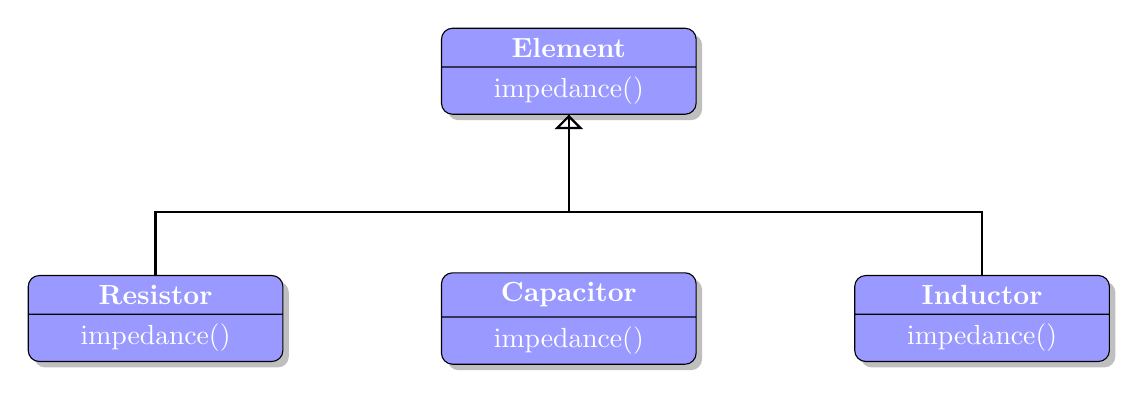
\begin{tikzpicture}[node distance=2cm]
    \node (Element) [abstract, rectangle split, rectangle split parts=2]
        {
            \textbf{Element}
            \nodepart{second}impedance()
        };

		\node (Capacitor) [abstract, rectangle split, rectangle split parts=2, below=of Element]
        {
            \textbf{Capacitor}
            \nodepart{second}impedance()
        };

    \node (Resistor) [abstract, rectangle split, rectangle split parts=2, left=of Capacitor]
        {
            \textbf{Resistor}
            \nodepart{second}impedance()
        };



    \node (Inductor) [abstract, rectangle split, rectangle split parts=2, right=of Capacitor]
        {
            \textbf{Inductor}
            \nodepart{second}impedance()
        };
    
    \draw[myarrow] (Resistor.north) -- ++(0,0.8) -| (Element.south);
    \draw[line] (Inductor.north) -- ++(0,0.8) -| (Element.south);
    
   % \draw[myarrow] (Sensor.north) -- ++(0,0.8) -| (Component.south);
    %\draw[line] (Sensor.north) -- ++(0,0.8) -| (Part.north);
    
   % \draw[line] (Pressure.west) -- ++(-0.2,0);
    %\draw[line] (Temperature.east) -- ++(0.2,0);
    %\draw[line] (Level.east) -- ++(0.2,0);
    %\draw[myarrow] (ClOp.west) -- ++(-0.2,0) -- ([yshift=0.5cm, xshift=-0.2cm] Pressure.north west) -|
    % ([xshift=-1cm]Sensor.south);
    %\draw[myarrow] (Ammeter.east) -- ++(0.2,0) -- ([yshift=0.5cm, xshift=0.2cm] Temperature.north east) -|
     %([xshift=1cm]Sensor.south);
     
    %\draw[line] (Tank.west) -- ++(-0.2,0);
    %\draw[line] (HeatExchanger.west) -- ++(-0.2,0);
    %\draw[line] (Pump.west) -- ++(-0.2,0);
    %\draw[line] (Valve.east) -- ++(0.2,0);
    %\draw[line] (Engine.east) -- ++(0.2,0);
    %\draw[myarrow] (Strainer.west) -- ++(-0.2,0) -- ([yshift=0.5cm, xshift=-0.2cm] Pump.north west) -|
     %([xshift=-1cm]Part.south);
    %\draw[myarrow] (Coolant.east) -- ++(0.2,0) -- ([yshift=0.5cm, xshift=0.2cm] Valve.north east) -|
     %([xshift=1cm]Part.south);
     
    %\draw[myarrow] (CoolingSystem.north) -- ++(0,0.8) -| (System.south);
    %\draw[line] (CoolingSystem.north) -- ++(0,0.8) -| (CoolingLoop.north);
        
        
\end{tikzpicture}